%%%%%%%%%%%%%%%%%%%%%%%%%%%%%%%%%%%%%%%%%%%%%%%%%%%%%%%%%%%%%%%%%%%%%%%%%%%%%%%%%%
\begin{frame}[fragile]\frametitle{}
\begin{center}
{\Large Overview of Generative AI}
\end{center}

{\tiny (Ref: 2023 Kaggle AI Report on Generative AI, by Trushant Kalyanpur)}

\end{frame}

%%%%%%%%%%%%%%%%%%%%%%%%%%%%%%%%%%%%%%%%%%%%%%%%%%%%%%%%%%%
\begin{frame}[fragile]\frametitle{Background: Advancements in Generative AI}
    
    \begin{itemize}
        \item Significance of Generative Pre-trained Transformer (GPT)
        \item GPT: Family of large-scale language models by OpenAI
        \item GPT architecture based on Transformer
        \item Transformer: Classic encoder-decoder architecture
        \item Encoder processes input, decoder generates output
    \end{itemize}
\end{frame}

%%%%%%%%%%%%%%%%%%%%%%%%%%%%%%%%%%%%%%%%%%%%%%%%%%%%%%%%%%%
\begin{frame}[fragile]\frametitle{Background: GPT Architecture}

\begin{itemize}
        \item GPT based on Transformer
        \item GPT uses stack of decoders
        \item Inspired by "Generating Wikipedia by Summarizing Long Sequences"
        \item Alternate arrangement of transformer block
        \item Model uses only stack of decoders
        \item GPT models are autoregressive
        \item Predicts next value based on previous values
        \item Sequence prediction mechanism
        \item Model predicts next value in a sequence
        \item Utilizes information from prior values		
\end{itemize}	

\begin{center}
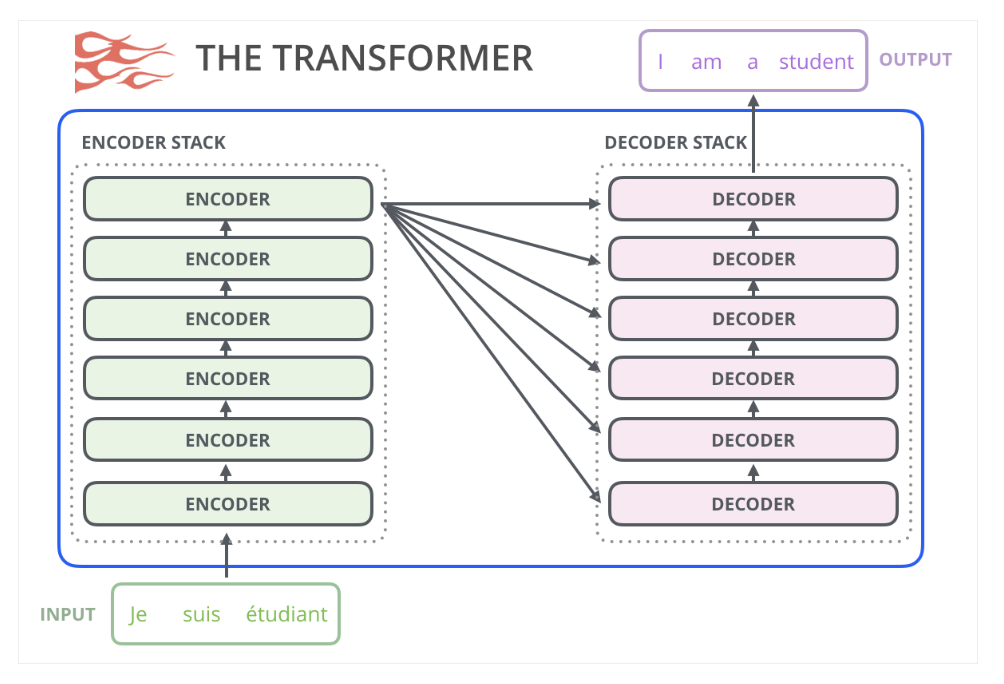
\includegraphics[width=0.6\linewidth,keepaspectratio]{llm85}
\end{center}		

\end{frame}

%%%%%%%%%%%%%%%%%%%%%%%%%%%%%%%%%%%%%%%%%%%%%%%%%%%%%%%%%%%
\begin{frame}[fragile]\frametitle{Background: GPT Architecture}

\begin{itemize}
        \item GPT based on Transformer
        \item GPT uses stack of decoders
        \item Inspired by "Generating Wikipedia by Summarizing Long Sequences"
        \item Alternate arrangement of transformer block
        \item Model uses only stack of decoders
        \item GPT models are autoregressive
        \item Predicts next value based on previous values
        \item Sequence prediction mechanism
        \item Model predicts next value in a sequence
        \item Utilizes information from prior values		
\end{itemize}	

\begin{center}
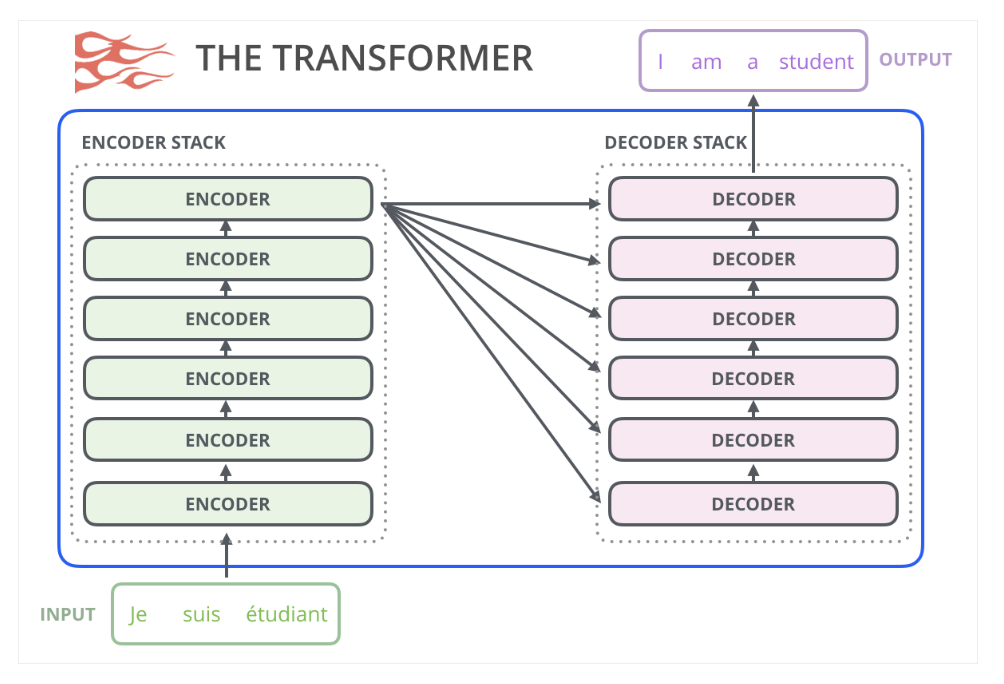
\includegraphics[width=0.6\linewidth,keepaspectratio]{llm85}
\end{center}		

{\tiny (Ref: Jay Alammar)}

\end{frame}

%%%%%%%%%%%%%%%%%%%%%%%%%%%%%%%%%%%%%%%%%%%%%%%%%%%%%%%%%%%
\begin{frame}[fragile]\frametitle{2021: Dall-E}

 Zero-Shot Text-to-Image Generation
 
\begin{itemize}
        \item OpenAI's 2021 release: DALL-E
        \item Text-to-image generation model
        \item Implementation of GPT-3
        \item Generates images from text descriptions
        \item Utilizes text-image dataset	
\end{itemize}	

\begin{center}
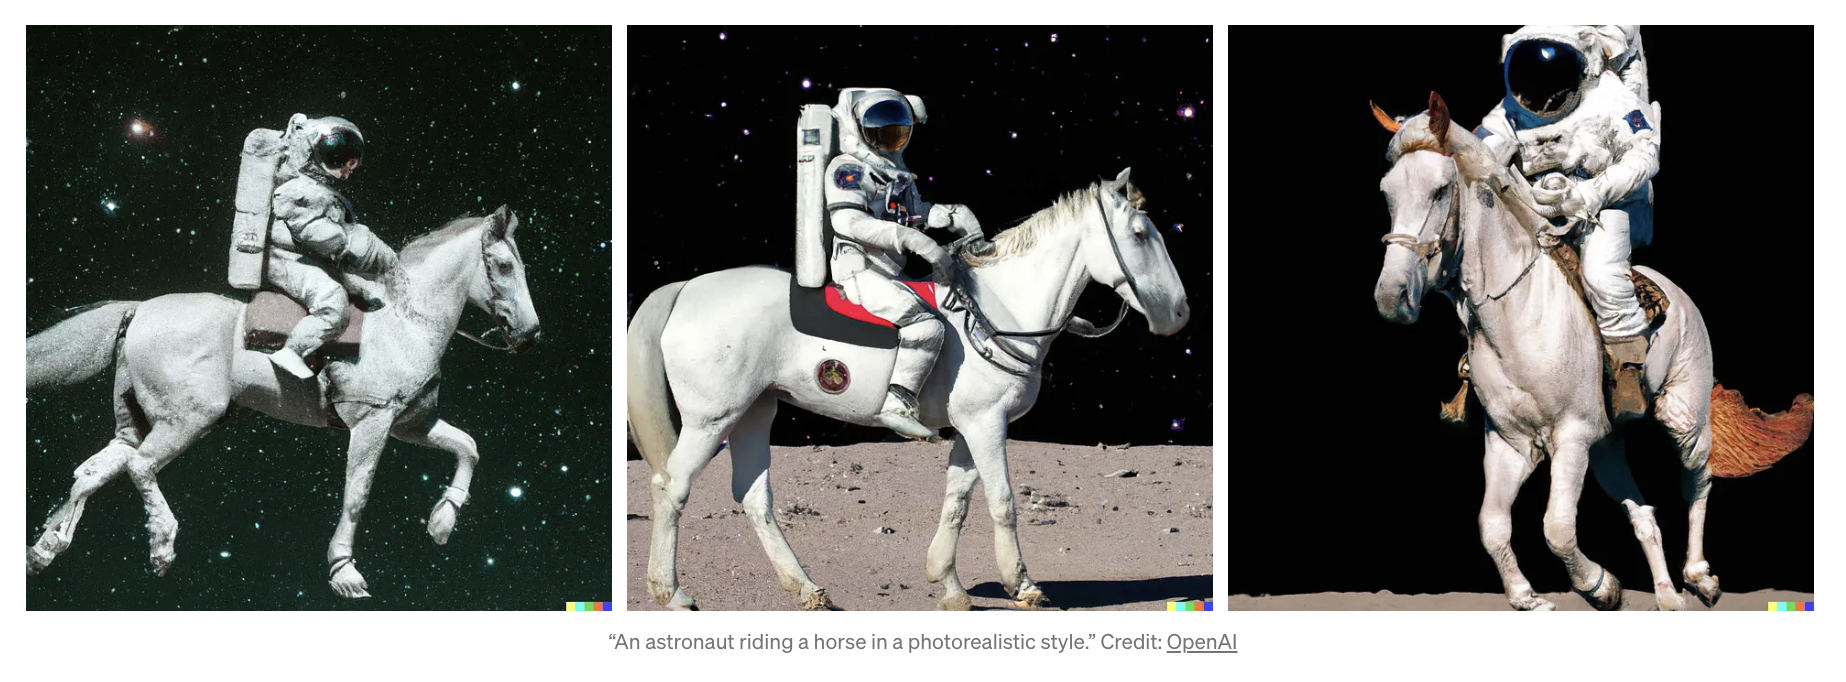
\includegraphics[width=0.6\linewidth,keepaspectratio]{llm86}
\end{center}		

{\tiny (Ref: Example prompt "An astronaut riding a horse in photorealistic style" using DALL-E: Open AI)}

\end{frame}

%%%%%%%%%%%%%%%%%%%%%%%%%%%%%%%%%%%%%%%%%%%%%%%%%%%%%%%%%%%
\begin{frame}[fragile]\frametitle{Contrastive Language-Image Pretraining (CLIP)}
    
    \begin{itemize}
        \item Revealed alongside DALL-E
        \item Trains model to understand text and images
        \item Learns coherent relationships between them
        \item Uses large-scale dataset (400 million pairs)
        \item Visual representations for downstream tasks
    \end{itemize}
\end{frame}

%%%%%%%%%%%%%%%%%%%%%%%%%%%%%%%%%%%%%%%%%%%%%%%%%%%%%%%%%%%
\begin{frame}[fragile]\frametitle{Integration of CLIP with DALL-E}
    
    \begin{itemize}
        \item CLIP evaluates DALL-E's output
        \item Analyzes suitable captions for generated images
        \item DALL-E's method: Inverted CLIP (unCLIP)
        \item Generates images from text
        \item Contrast to CLIP's image-to-text approach
    \end{itemize}
\end{frame}

%%%%%%%%%%%%%%%%%%%%%%%%%%%%%%%%%%%%%%%%%%%%%%%%%%%%%%%%%%%
\begin{frame}[fragile]\frametitle{Implications and Creativity}
    
    \begin{itemize}
        \item Concerns about creativity impact
        \item Worries for artists, designers, illustrators
        \item DALL-E generates intricate images
        \item Sparks creativity and new ideas
        \item Benefits storytelling, concept art, expression
    \end{itemize}
\end{frame}


%%%%%%%%%%%%%%%%%%%%%%%%%%%%%%%%%%%%%%%%%%%%%%%%%%%%%%%%%%%
\begin{frame}[fragile]\frametitle{Github Copilot: Breakthrough Coding Assistant}
    
    \begin{itemize}
        \item OpenAI introduced Github Copilot in 2021
        \item Built on GPT-3 architecture
        \item Fine-tuned on millions of public code lines
        \item Auto-completes and suggests code
        \item Supports multiple programming languages
    \end{itemize}
\end{frame}

%%%%%%%%%%%%%%%%%%%%%%%%%%%%%%%%%%%%%%%%%%%%%%%%%%%%%%%%%%%
\begin{frame}[fragile]\frametitle{Concerns and Considerations}
    
    \begin{itemize}
        \item Raised intellectual property rights issues
        \item Trained on publicly available GitHub code
        \item Potential licensing conflicts
        \item Risk of suggesting code with vulnerabilities
        \item Biases and security flaws in training data
    \end{itemize}
\end{frame}

%%%%%%%%%%%%%%%%%%%%%%%%%%%%%%%%%%%%%%%%%%%%%%%%%%%%%%%%%%%
\begin{frame}[fragile]\frametitle{Impact on Developer Community}
    
    \begin{itemize}
        \item Enhanced productivity among developers
        \item Focus on higher-level tasks and problem-solving
        \item Reduced time spent on repetitive code
        \item Empowers creativity and innovation
        \item New perspectives in software development
    \end{itemize}
\end{frame}

%%%%%%%%%%%%%%%%%%%%%%%%%%%%%%%%%%%%%%%%%%%%%%%%%%%%%%%%%%%
\begin{frame}[fragile]\frametitle{2022: Pathways Language Model (PaLM)}
    
    \begin{itemize}
        \item Developed by Google AI
        \item Large language model (LLM)
        \item 540B parameters (3x GPT-3's size)
        \item Aims for efficiency and scalability
        \item Achieves state-of-the-art performance
    \end{itemize}
\end{frame}

%%%%%%%%%%%%%%%%%%%%%%%%%%%%%%%%%%%%%%%%%%%%%%%%%%%%%%%%%%%
\begin{frame}[fragile]\frametitle{Pathways Architecture}
    
    \begin{itemize}
        \item Utilizes hierarchical Pathways
        \item Learns various abstraction levels
        \item Efficient and scalable design
        \item Scales training to thousands of TPU chips
        \item Combines data parallelism and model parallelism
    \end{itemize}
\end{frame}

%%%%%%%%%%%%%%%%%%%%%%%%%%%%%%%%%%%%%%%%%%%%%%%%%%%%%%%%%%%
\begin{frame}[fragile]\frametitle{Data and Training}
    
    \begin{itemize}
        \item Trained on 780 billion tokens
        \item Includes webpages, books, Wikipedia, news, code
        \item Filters diverse sources of data
        \item Enables broader language understanding
        \item Expands model's contextual knowledge
    \end{itemize}
\end{frame}

%%%%%%%%%%%%%%%%%%%%%%%%%%%%%%%%%%%%%%%%%%%%%%%%%%%%%%%%%%%
\begin{frame}[fragile]\frametitle{Performance and Achievements}
    
    \begin{itemize}
        \item Outperforms previous models
        \item Improvements across various tasks
        \item Enhanced text generation: factual and creative
        \item Improved question answering accuracy
        \item Fluent machine translation between languages
    \end{itemize}
\end{frame}

%%%%%%%%%%%%%%%%%%%%%%%%%%%%%%%%%%%%%%%%%%%%%%%%%%%%%%%%%%%
\begin{frame}[fragile]\frametitle{DALL-E 2: Successor to DALL-E}
    
    \begin{itemize}
        \item OpenAI released DALL-E 2 in April 2022
        \item Builds upon DALL-E's foundation
        \item Uses CLIP embeddings directly
        \item Decodes images with a diffusion model
        \item Shift from decoder-only transformer
    \end{itemize}
\end{frame}

%%%%%%%%%%%%%%%%%%%%%%%%%%%%%%%%%%%%%%%%%%%%%%%%%%%%%%%%%%%
\begin{frame}[fragile]\frametitle{Diffusion Model in DALL-E 2}
    
    \begin{itemize}
        \item Diffusion model for image generation
        \item Gradually adds noise to match text
        \item Avoids one-pixel-at-a-time limitation
        \item Produces more realistic images
        \item Improves image quality and coherence
    \end{itemize}
	
\begin{center}
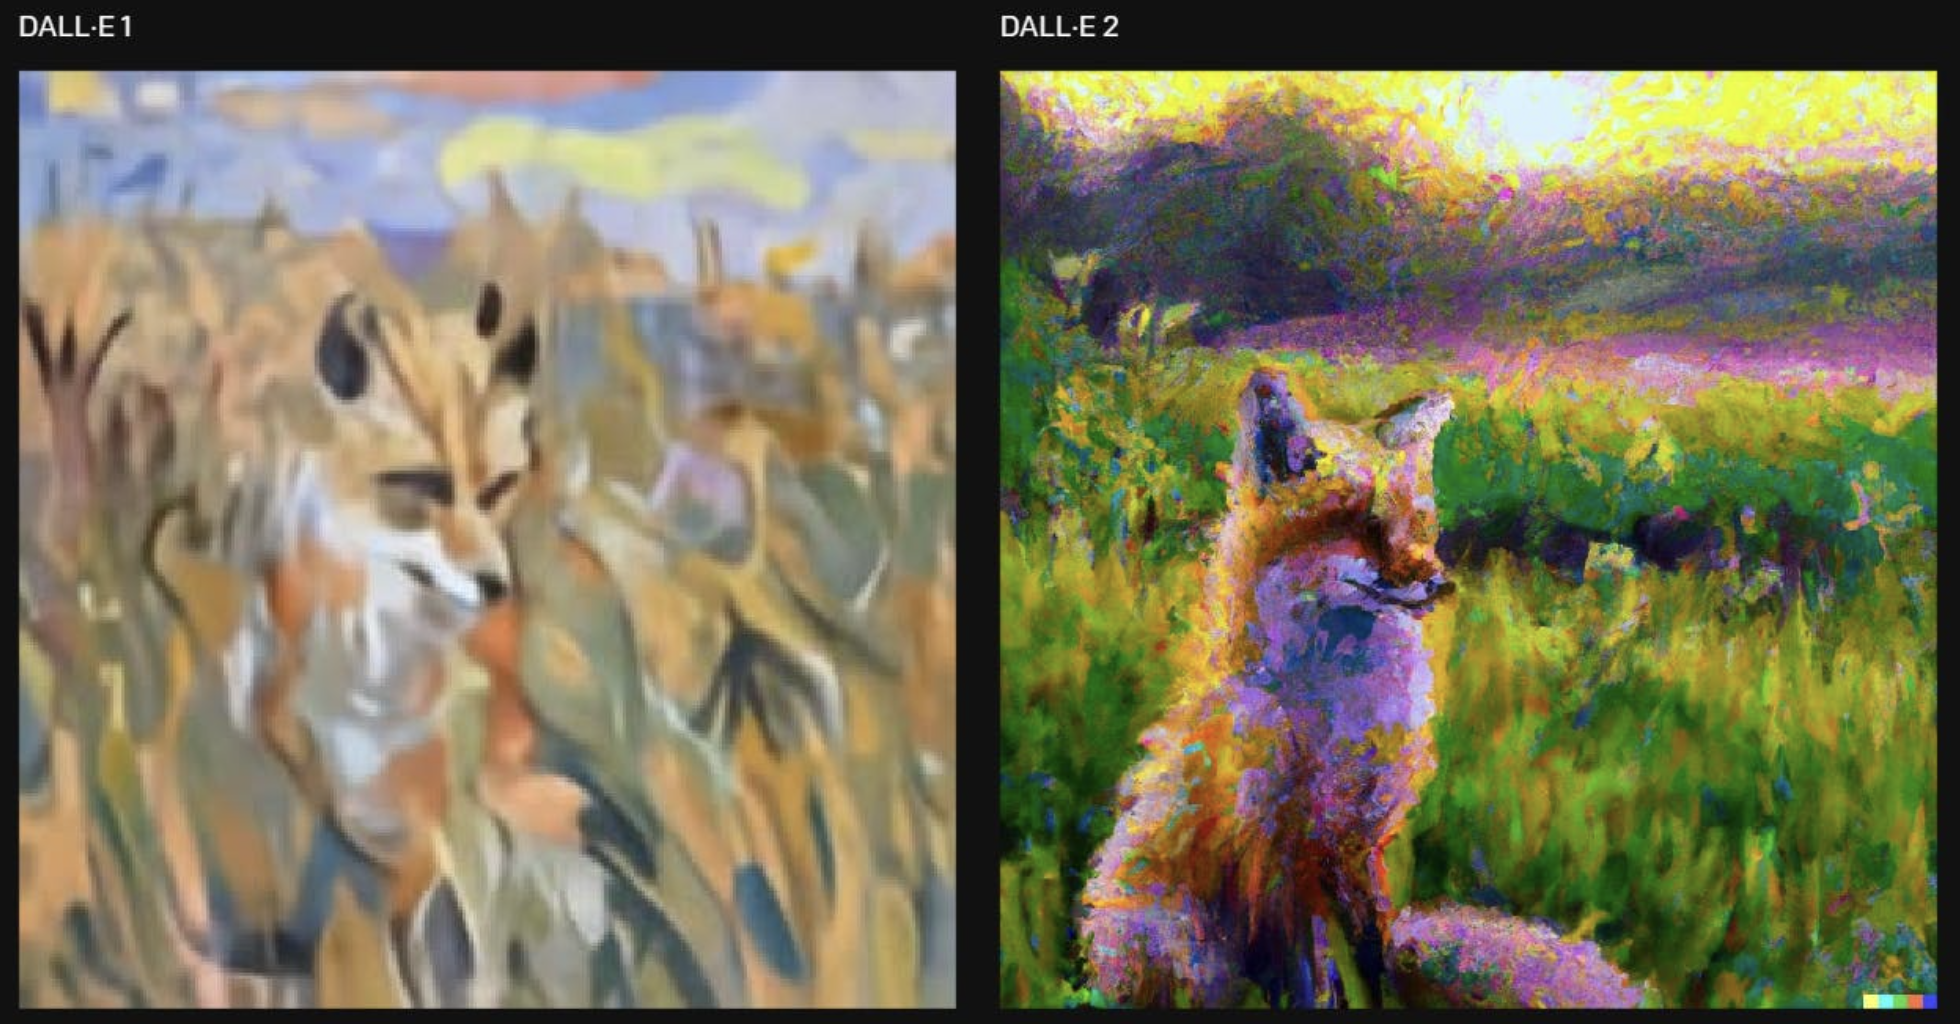
\includegraphics[width=0.6\linewidth,keepaspectratio]{llm87}
\end{center}		

{\tiny (Ref: Same prompt: "a painting of a fox sitting in a field at sunrise in the style of Claude Monet": Open AI)}
	
\end{frame}

%%%%%%%%%%%%%%%%%%%%%%%%%%%%%%%%%%%%%%%%%%%%%%%%%%%%%%%%%%%
\begin{frame}[fragile]\frametitle{CLIP Training and Generation}
    
    \begin{itemize}
        \item Joint representation space for text and images
        \item Text-to-image process with CLIP text embedding
        \item Autoregressive or diffusion prior
        \item Image embedding for diffusion decoder
        \item Diffusion decoder generates final image
    \end{itemize}
\end{frame}

%%%%%%%%%%%%%%%%%%%%%%%%%%%%%%%%%%%%%%%%%%%%%%%%%%%%%%%%%%%
\begin{frame}[fragile]\frametitle{Improved Realism in DALL-E 2}
    
    \begin{itemize}
        \item Enhanced image generation quality
        \item CLIP embeddings, diffusion prior, decoder
        \item Realistic and accurate images
        \item Advances over DALL-E's capabilities
        \item Notable improvement in image fidelity
    \end{itemize}
\end{frame}

%%%%%%%%%%%%%%%%%%%%%%%%%%%%%%%%%%%%%%%%%%%%%%%%%%%%%%%%%%%
\begin{frame}[fragile]\frametitle{Image Quality Comparison}
    
    \begin{itemize}
        \item Example: "painting of a fox at sunrise"
        \item DALL-E 2 vs DALL-E
        \item Image quality and style differences
        \item Enhanced fidelity and style representation
        \item Demonstrates DALL-E 2's advancements
    \end{itemize}
\end{frame}

%%%%%%%%%%%%%%%%%%%%%%%%%%%%%%%%%%%%%%%%%%%%%%%%%%%%%%%%%%%
\begin{frame}[fragile]\frametitle{Midjourney: Image Generation Model}
    
    \begin{itemize}
        \item Developed by Midjourney Inc.
        \item Released in July 2022
        \item Architecture details undisclosed
        \item High-quality image generation
        \item Wide variety of styles and genres
    \end{itemize}
	
\end{frame}

%%%%%%%%%%%%%%%%%%%%%%%%%%%%%%%%%%%%%%%%%%%%%%%%%%%%%%%%%%%
\begin{frame}[fragile]\frametitle{Open Beta Access}
    
    \begin{itemize}
        \item Released in open beta via Discord
        \item Anyone could sign up and use
        \item High accessibility for image generation
        \item Among the most accessible LLMs
        \item Democratizing image creation process
    \end{itemize}
\end{frame}

%%%%%%%%%%%%%%%%%%%%%%%%%%%%%%%%%%%%%%%%%%%%%%%%%%%%%%%%%%%
\begin{frame}[fragile]\frametitle{Evolution of Midjourney Images}
    
    \begin{itemize}
        \item Image quality improvement over time
        \item Different versions of Midjourney
        \item Same prompt for image generation
        \item Version range from 1 to 5
        \item Released between 2022 and March 2023
    \end{itemize}
\end{frame}

%%%%%%%%%%%%%%%%%%%%%%%%%%%%%%%%%%%%%%%%%%%%%%%%%%%%%%%%%%%
\begin{frame}[fragile]\frametitle{Progressive Image Enhancement}
    
    \begin{itemize}
        \item Comparison across Midjourney versions
        \item Images generated with same prompt
        \item Version 5 (March 2023) > Version 1 (2022)
        \item Newer versions: more detailed, realistic, creative
        \item Evident improvements in image quality
    \end{itemize}
	
\begin{center}
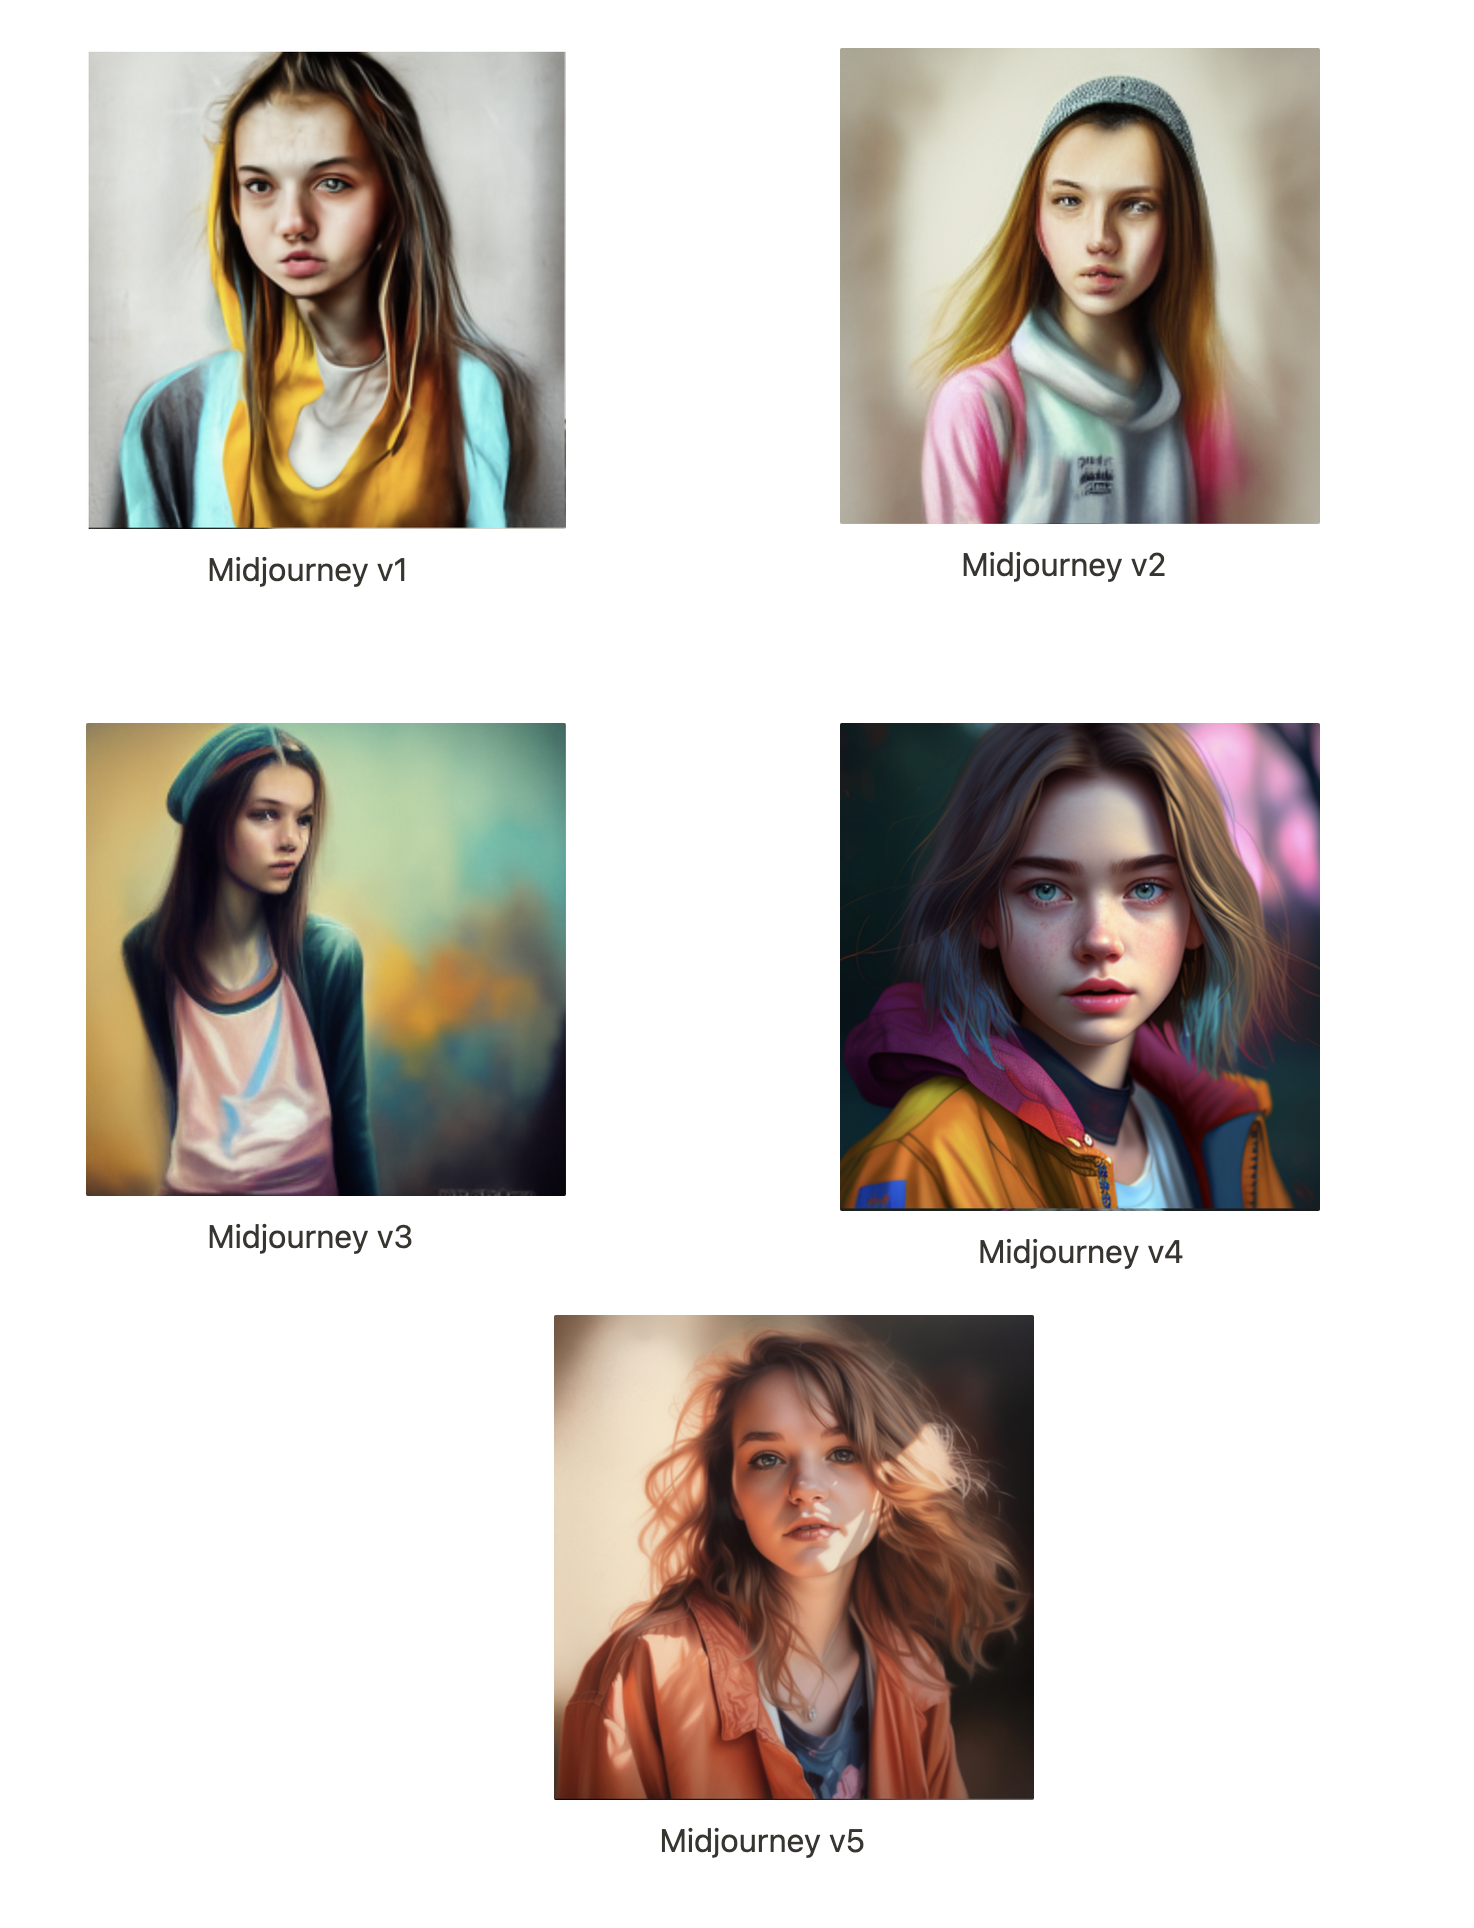
\includegraphics[width=0.4\linewidth,keepaspectratio]{llm88}
\end{center}		

{\tiny (Ref: Prompt: Teenager, female, seventeen years old, pop culture, modern clothing. Photorealistic, Natural lighting, Pastel. Image credit John Severinson)}
		
\end{frame}


%%%%%%%%%%%%%%%%%%%%%%%%%%%%%%%%%%%%%%%%%%%%%%%%%%%%%%%%%%%
\begin{frame}[fragile]\frametitle{Stable Diffusion: Latent Image Generation}
    
    \begin{itemize}
        \item Released in August 2022
        \item Latent diffusion model
        \item Generates images from text descriptions
        \item Notable contribution to open source LLMs
        \item Developed by CompVis Group, Ludwig Maximilian University
    \end{itemize}

\end{frame}

%%%%%%%%%%%%%%%%%%%%%%%%%%%%%%%%%%%%%%%%%%%%%%%%%%%%%%%%%%%
\begin{frame}[fragile]\frametitle{Stable Diffusion: Latent Image Generation}
    
    \begin{itemize}
        \item ClipText for text encoding - This takes in a text and outputs the text embedding vectors.
        \item Diffusion: UNet + Scheduler to gradually process/diffuse information in the information (latent) space - This block takes in the text embeddings and an initial tensor made up of noise. It outputs a processed information array.
        \item Autoencoder Decoder - This decoder paints the final image using the processed information array.
    \end{itemize}
	
\begin{center}
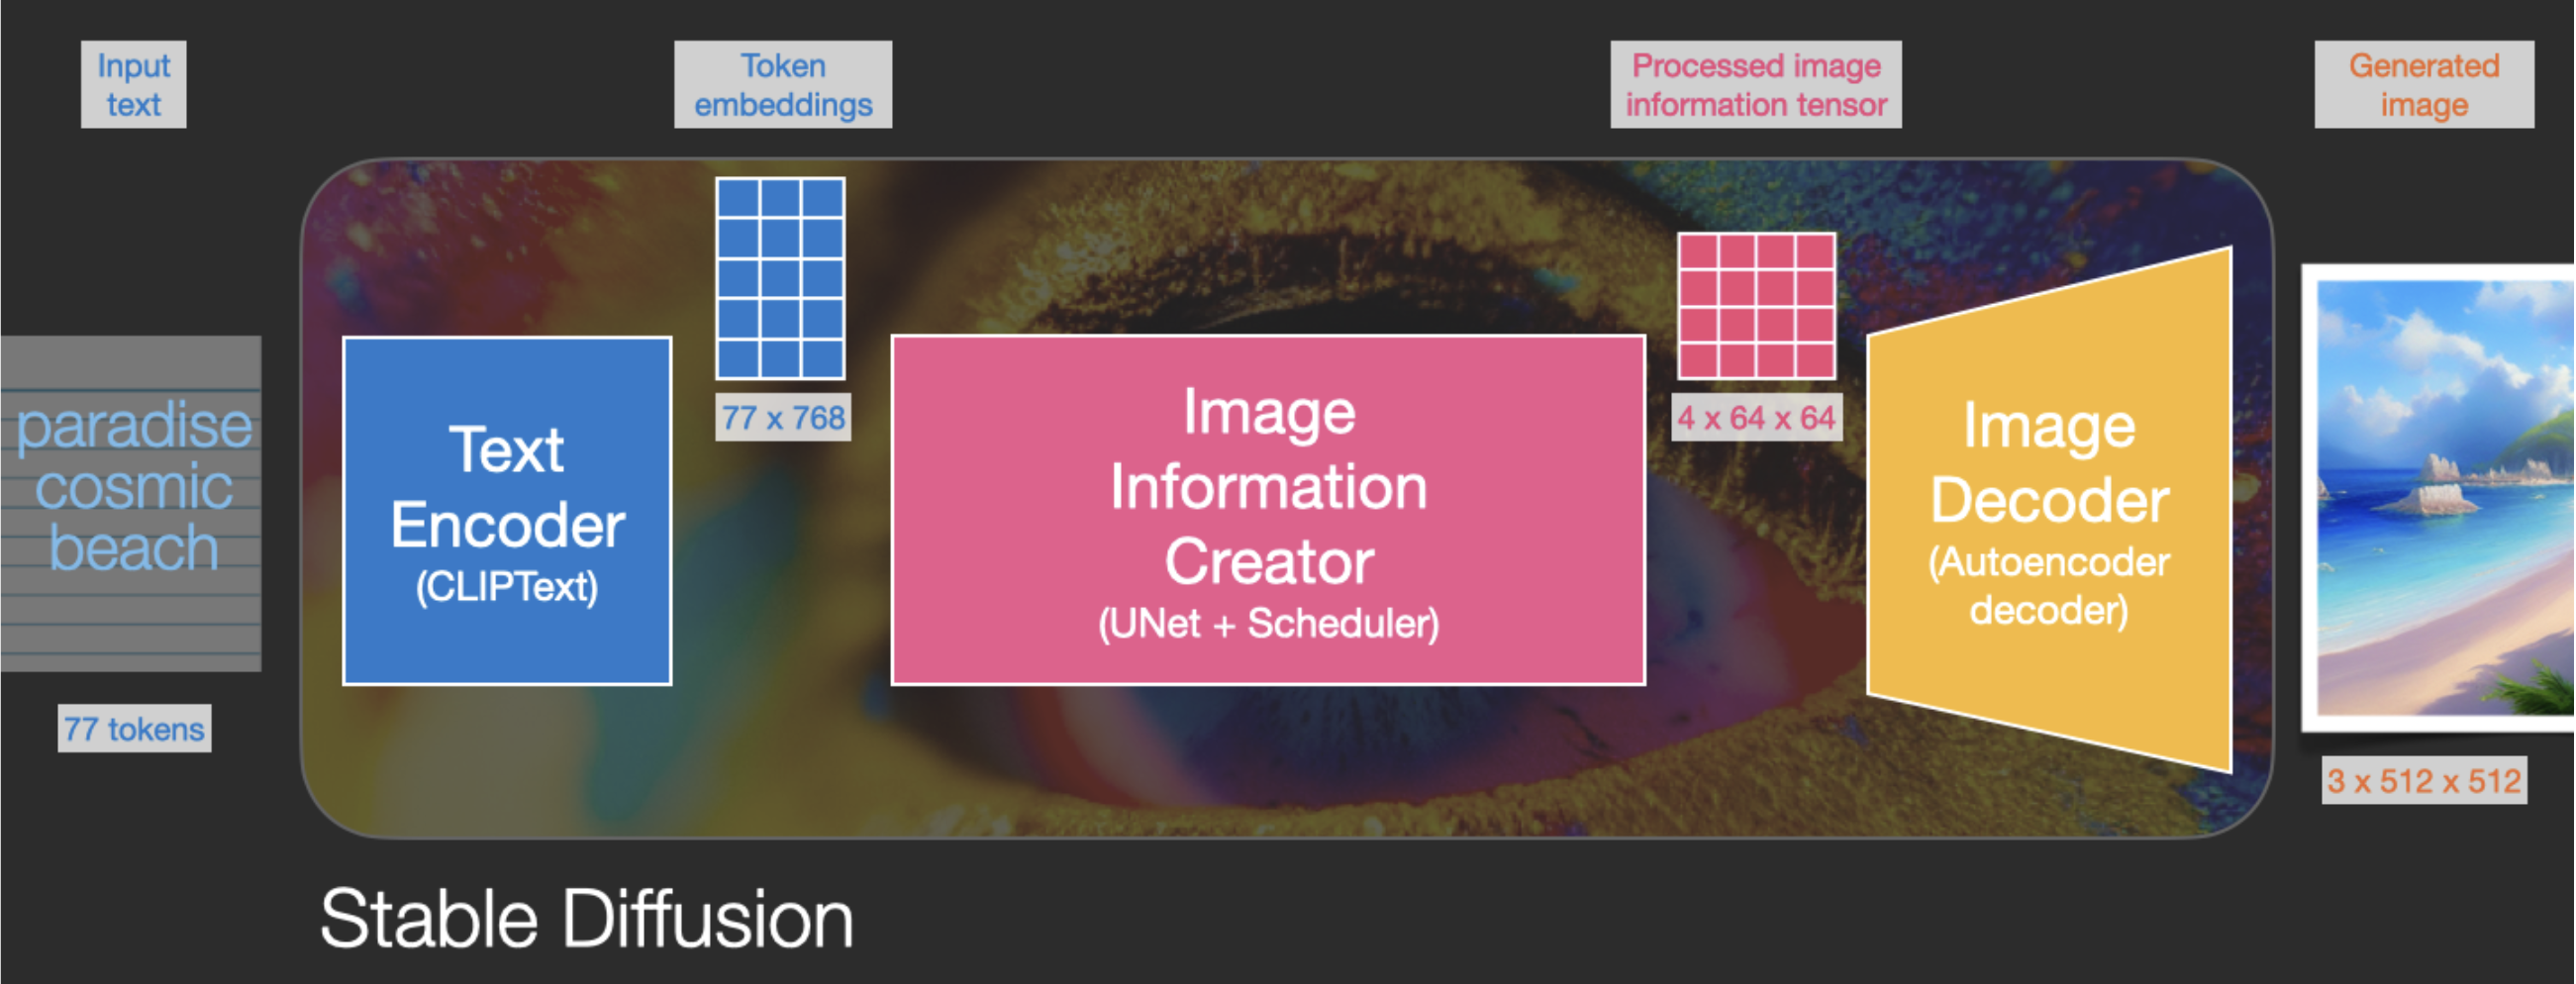
\includegraphics[width=0.6\linewidth,keepaspectratio]{llm89}
\end{center}		

{\tiny (Ref: Jay Alammar)}
		
\end{frame}

%%%%%%%%%%%%%%%%%%%%%%%%%%%%%%%%%%%%%%%%%%%%%%%%%%%%%%%%%%%
\begin{frame}[fragile]\frametitle{Open Source Impact}
    
    \begin{itemize}
        \item Code and model weights released publicly
        \item One of the earliest open source LLMs for image generation
        \item Focus on generating images from text
        \item Enhances accessibility and collaboration
        \item Advancement in sharing research and tools
    \end{itemize}
\end{frame}

%%%%%%%%%%%%%%%%%%%%%%%%%%%%%%%%%%%%%%%%%%%%%%%%%%%%%%%%%%%
\begin{frame}[fragile]\frametitle{Latent Diffusion Model}
    
    \begin{itemize}
        \item Uses latent space for image representation
        \item Generates images from noisy inputs
        \item Gradually reduces noise for realism
        \item More diverse and creative image generation
        \item Contrasts with traditional diffusion models
    \end{itemize}
\end{frame}

%%%%%%%%%%%%%%%%%%%%%%%%%%%%%%%%%%%%%%%%%%%%%%%%%%%%%%%%%%%
\begin{frame}[fragile]\frametitle{Collaborative Development}
    
    \begin{itemize}
        \item Collaboration between institutions
        \item Developed by CompVis Group and Runway
        \item Compute donation by Stability AI
        \item Training data from non-profit organizations
        \item Cross-disciplinary efforts for innovation
    \end{itemize}
\end{frame}

%%%%%%%%%%%%%%%%%%%%%%%%%%%%%%%%%%%%%%%%%%%%%%%%%%%%%%%%%%%
\begin{frame}[fragile]\frametitle{ChatGPT - A Tipping Point for Generative AI}
    \begin{itemize}
        \item Released by OpenAI in November 2022
        \item Generative AI chatbot
        \item Rapid worldwide popularity
        \item 1 million users in 5 days
        \item Netflix took 3.5 years for same user count
        \item 100 million monthly active users by January 2023
        \item Fastest-growing application in history
    \end{itemize}
\end{frame}

%%%%%%%%%%%%%%%%%%%%%%%%%%%%%%%%%%%%%%%%%%%%%%%%%%%%%%%%%%%
\begin{frame}[fragile]\frametitle{Versatile Capabilities of ChatGPT}
    \begin{itemize}
        \item Generates human-like chat conversations
        \item Tasks: questions, creative content, explanations
        \item Suggestions, poems, code generation, and more
    \end{itemize}
\end{frame}

%%%%%%%%%%%%%%%%%%%%%%%%%%%%%%%%%%%%%%%%%%%%%%%%%%%%%%%%%%%
\begin{frame}[fragile]\frametitle{Pivotal Moment in AI}
    \begin{itemize}
        \item Demonstrated advanced language model sophistication
        \item Prompted activity in AI community
        \item Rush to develop similar language models
        \item Expectation of even more impressive models
    \end{itemize}
\end{frame}

%%%%%%%%%%%%%%%%%%%%%%%%%%%%%%%%%%%%%%%%%%%%%%%%%%%%%%%%%%%
\begin{frame}[fragile]\frametitle{Technical Details - ChatGPT}
    \begin{itemize}
        \item Based on GPT3 architecture
        \item Estimated 175 billion parameters
        \item Fine-tuned on chat-specific task
        \item Curated dataset for fine-tuning
        \item Human AI trainers provide feedback
        \item Model adjusts responses based on feedback
    \end{itemize}
\end{frame}

%%%%%%%%%%%%%%%%%%%%%%%%%%%%%%%%%%%%%%%%%%%%%%%%%%%%%%%%%%%
\begin{frame}[fragile]\frametitle{Specialization Through Fine-tuning}
    \begin{itemize}
        \item Specializes in domains or tasks
        \item Incorporates human preferences and guidelines
        \item Examples: conversational data, customer support
        \item More suitable for interactive applications
    \end{itemize}
\end{frame}

%%%%%%%%%%%%%%%%%%%%%%%%%%%%%%%%%%%%%%%%%%%%%%%%%%%%%%%%%%%
\begin{frame}[fragile]\frametitle{Improving ChatGPT with RLHF}
    \begin{itemize}
        \item Key technique: Reinforcement Learning from Human Feedback (RLHF)
        \item Trains language model to align with human preferences
        \item Collects human feedback on model-generated text
        \item Updates model's parameters using feedback
        \item Enhances ChatGPT responses' quality
        \item Increases factual, informative, and creative output
    \end{itemize}
\end{frame}

%%%%%%%%%%%%%%%%%%%%%%%%%%%%%%%%%%%%%%%%%%%%%%%%%%%%%%%%%%%
\begin{frame}[fragile]\frametitle{ChatGPT's Impact on Generative AI}
    \begin{itemize}
        \item Represents a tipping point for generative AI
        \item Demonstrates capability of Language Models (LLMs)
        \item LLMs generate human-quality chat conversations
        \item Expands LLM applications across various domains
    \end{itemize}
\end{frame}

%%%%%%%%%%%%%%%%%%%%%%%%%%%%%%%%%%%%%%%%%%%%%%%%%%%%%%%%%%%
\begin{frame}[fragile]\frametitle{Raising Awareness and Potential}
    \begin{itemize}
        \item ChatGPT's popularity contributes to raising awareness
        \item Highlights potential benefits of generative AI
        \item Opens doors to innovative applications
    \end{itemize}
\end{frame}


%%%%%%%%%%%%%%%%%%%%%%%%%%%%%%%%%%%%%%%%%%%%%%%%%%%%%%%%%%%
\begin{frame}[fragile]\frametitle{Meta Releases LLaMA - Open Source LLMs Explode!}
    \begin{itemize}
        \item February 2023: Meta releases LLM "LLaMA"
        \item LLaMA: 65-billion parameter model
        \item Trained on extensive text and code dataset
    \end{itemize}
\end{frame}

%%%%%%%%%%%%%%%%%%%%%%%%%%%%%%%%%%%%%%%%%%%%%%%%%%%%%%%%%%%
\begin{frame}[fragile]\frametitle{Significance of LLaMA Release}
    \begin{itemize}
        \item One of the largest public LLMs
        \item Suited for complex and challenging tasks
        \item Open source, initially for research purposes
        \item Model weights leaked online, accessible to all
        \item Sparked development of numerous open source LLMs
    \end{itemize}
\end{frame}


%%%%%%%%%%%%%%%%%%%%%%%%%%%%%%%%%%%%%%%%%%%%%%%%%%%%%%%%%%%
\begin{frame}[fragile]\frametitle{Google Releases Bard}
    \begin{itemize}
        \item March 2023: Google introduces Bard chatbot
        \item Built on LLM framework
        \item Fine-tuned model based on PaLM 2
        \item PaLM 2: Around 340 billion parameters
        \item Bard trained on dataset 10 times larger than ChatGPT
    \end{itemize}
\end{frame}

%%%%%%%%%%%%%%%%%%%%%%%%%%%%%%%%%%%%%%%%%%%%%%%%%%%%%%%%%%%
\begin{frame}[fragile]\frametitle{Bard's Unique Features}
    \begin{itemize}
        \item Access to the internet
        \item Continuous learning and knowledge update
        \item More up-to-date and accurate than ChatGPT
        \item ChatGPT limited to training dataset info
        \item Bard surpasses ChatGPT's knowledge scope
    \end{itemize}
\end{frame}

%%%%%%%%%%%%%%%%%%%%%%%%%%%%%%%%%%%%%%%%%%%%%%%%%%%%%%%%%%%
\begin{frame}[fragile]\frametitle{QLoRA: Quantized LLMs with Low-Rank Adapters}
    \begin{itemize}
        \item May 2023: Dettmers et al. released QLoRA
        \item Built on 2021's LoRA by Hu et al.
        \item LoRA: Reduces LLM memory footprint with adapters
        \item Frozen original LLM parameters
        \item Adapter weights updated during fine-tuning
    \end{itemize}
	
\begin{center}
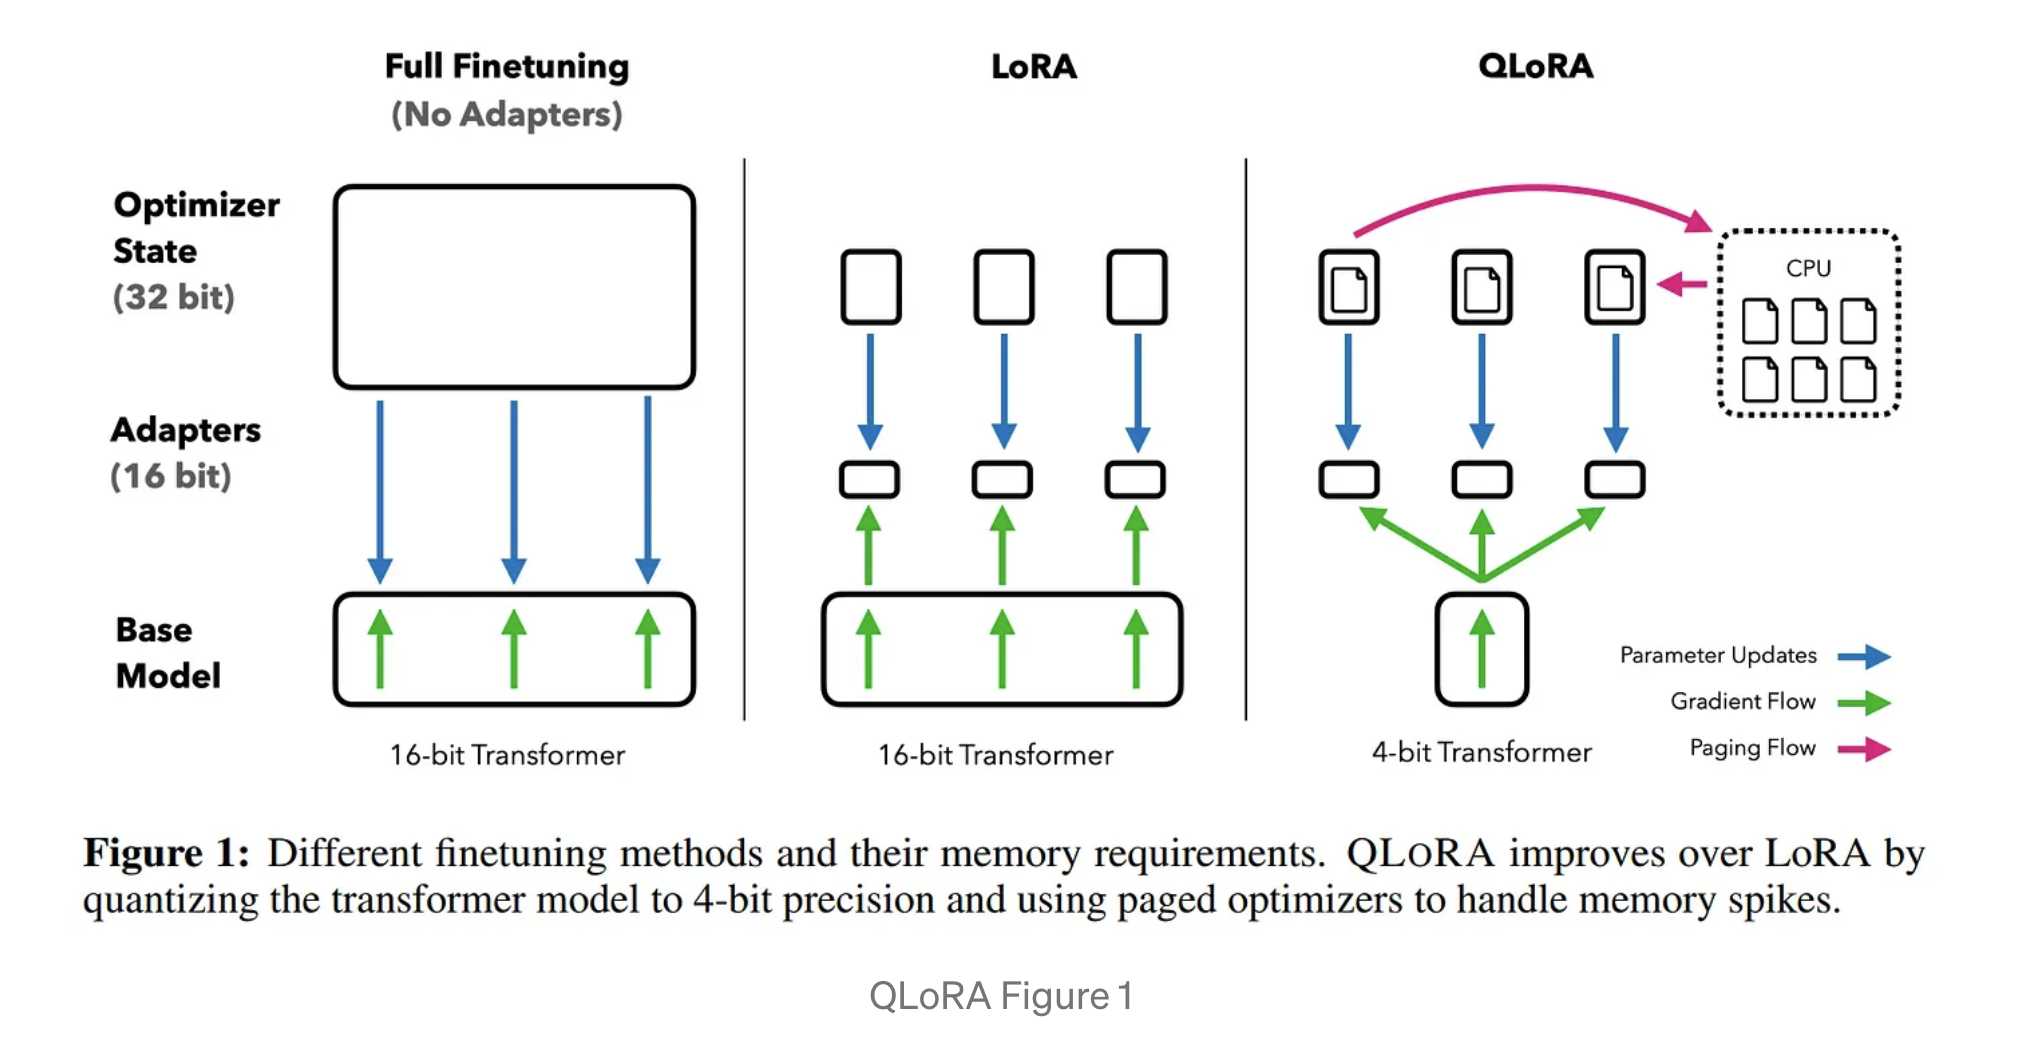
\includegraphics[width=0.6\linewidth,keepaspectratio]{llm90}
\end{center}		

{\tiny (Ref: QLoRA paper)}
			
\end{frame}

%%%%%%%%%%%%%%%%%%%%%%%%%%%%%%%%%%%%%%%%%%%%%%%%%%%%%%%%%%%
\begin{frame}[fragile]\frametitle{QLoRA's Innovations}
    \begin{itemize}
        \item Extension of LoRA technique
        \item Introduces 4-bit quantization
        \item Double quantization and paged optimizers
        \item Utilizes Nvidia's unified memory for paging
        \item Drastic memory reduction in 65B model finetuning
    \end{itemize}
\end{frame}

%%%%%%%%%%%%%%%%%%%%%%%%%%%%%%%%%%%%%%%%%%%%%%%%%%%%%%%%%%%
\begin{frame}[fragile]\frametitle{Benefits and Impact}
    \begin{itemize}
        \item Enables finetuning on limited resources
        \item 65B model on a single 48GB GPU
        \item Maintains full 16-bit finetuning performance
        \item Essential for pretrained LLMs' ChatGPT-like capabilities
        \item Expands accessibility to state-of-the-art NLP technology
    \end{itemize}
\end{frame}

%%%%%%%%%%%%%%%%%%%%%%%%%%%%%%%%%%%%%%%%%%%%%%%%%%%%%%%%%%%
\begin{frame}[fragile]\frametitle{OpenAI Releases GPT4}
    \begin{itemize}
        \item May 2023: OpenAI releases GPT4
        \item Multimodal: accepts image and text inputs
        \item Generates text outputs
        \item 6 months spent on safety and alignment
        \item GPT-4 82% less likely for disallowed content
        \item 40% more likely for factual responses than GPT-3.5
    \end{itemize}
\end{frame}

%%%%%%%%%%%%%%%%%%%%%%%%%%%%%%%%%%%%%%%%%%%%%%%%%%%%%%%%%%%
\begin{frame}[fragile]\frametitle{GPT4's Performance}
    \begin{itemize}
        \item Human-level performance on benchmarks
        \item Passed simulated bar exam in top 10%
        \item Impressive results on various professional exams
        \item Chart compares GPT4 and GPT3.5 performance
    \end{itemize}
\end{frame}

%%%%%%%%%%%%%%%%%%%%%%%%%%%%%%%%%%%%%%%%%%%%%%%%%%%%%%%%%%%
\begin{frame}[fragile]\frametitle{GPT4's Architecture}
    \begin{itemize}
        \item Rumored architecture: eight models with 220B parameters
        \item Linked in Mixture of Experts (MoE) structure
        \item Total model: 1.76T parameters
        \item MoE combines different "experts" for decision making
        \item Enabling complex and diverse capabilities
    \end{itemize}
\end{frame}